\documentclass[xcolor=dvipsnames, handout, mathserif]{beamer} 

%% Layout and definitions
\usepackage{import}
\import{../../Layout/}{slide_layout.tex}
\import{../../Layout/}{definitions.tex}

%% Front page and content
\title{MS-E2122 - Nonlinear Optimization \\ Lecture 1}
\date{\today}
\author{Fabricio Oliveira}
\institute{Systems Analysis Laboratory \\ Department of Mathematics and Systems Analysis \vskip 0.25cm 
           Aalto University\\
           School of Science}

%% Begin of the file
\begin{document}

\begin{frame}[noframenumbering]
    \thispagestyle{empty}
    \titlepage
\end{frame}

\begin{frame}
%	\thispagestyle{empty}
	\frametitle{Outline of this lecture} 
	\tableofcontents
\end{frame} 

%% Slide content
\addtocounter{framenumber}{-1}
\section{What is optimisation?}


\begin{frame}{What is optimisation?}

	Discipline of applied mathematics. The idea is to search values for \alert{variables}\hspace{-1pt} in a given \alert{domain} that\hspace{-1pt} maximise/minimise\hspace{-1pt} \alert{function values}. 
	
	Can be achieved by 
	\begin{itemize}[<+->]
	\item Analysing properties of functions \hspace{-1pt}/ extreme points or
	\item Applying numerical methods 
	\end{itemize}
	\onslide<+->
	
	Optimisation has important applications in fields such as 
	%
	\begin{itemize}
	\item {\bf operations research (OR)};
	\item economics;
	\item statistics; 
	\item machine learning and artificial intelligence.
	\end{itemize}

\end{frame}


\subsection{Mathematical programming and optimisation}


\begin{frame}{What is optimisation?}

	In this course, optimisation is viewed as the core element of \alert{mathematical programming}.
	
	Math. programming is a central OR modelling paradigm:
	\begin{itemize}[<+->]
	\item {\bf variables} $\rightarrow$ decisions: business decisions, parameter definitions, settings, geometries, ...;
	\item {\bf domain} $\rightarrow$ constraints: logic, design, engineering, ...;
	\item {\bf function} $\rightarrow$ objective function: measurement of (decision) quality. 
	\end{itemize}
	
	\onslide<+->
	However, math. programming has many applications in fields other than OR, \alert{which causes some confusion}; 
	
	We will study math. programming in its most general form: both constraints and objectives are \alert{nonlinear} functions.

\end{frame}


\begin{frame}
	\centering
	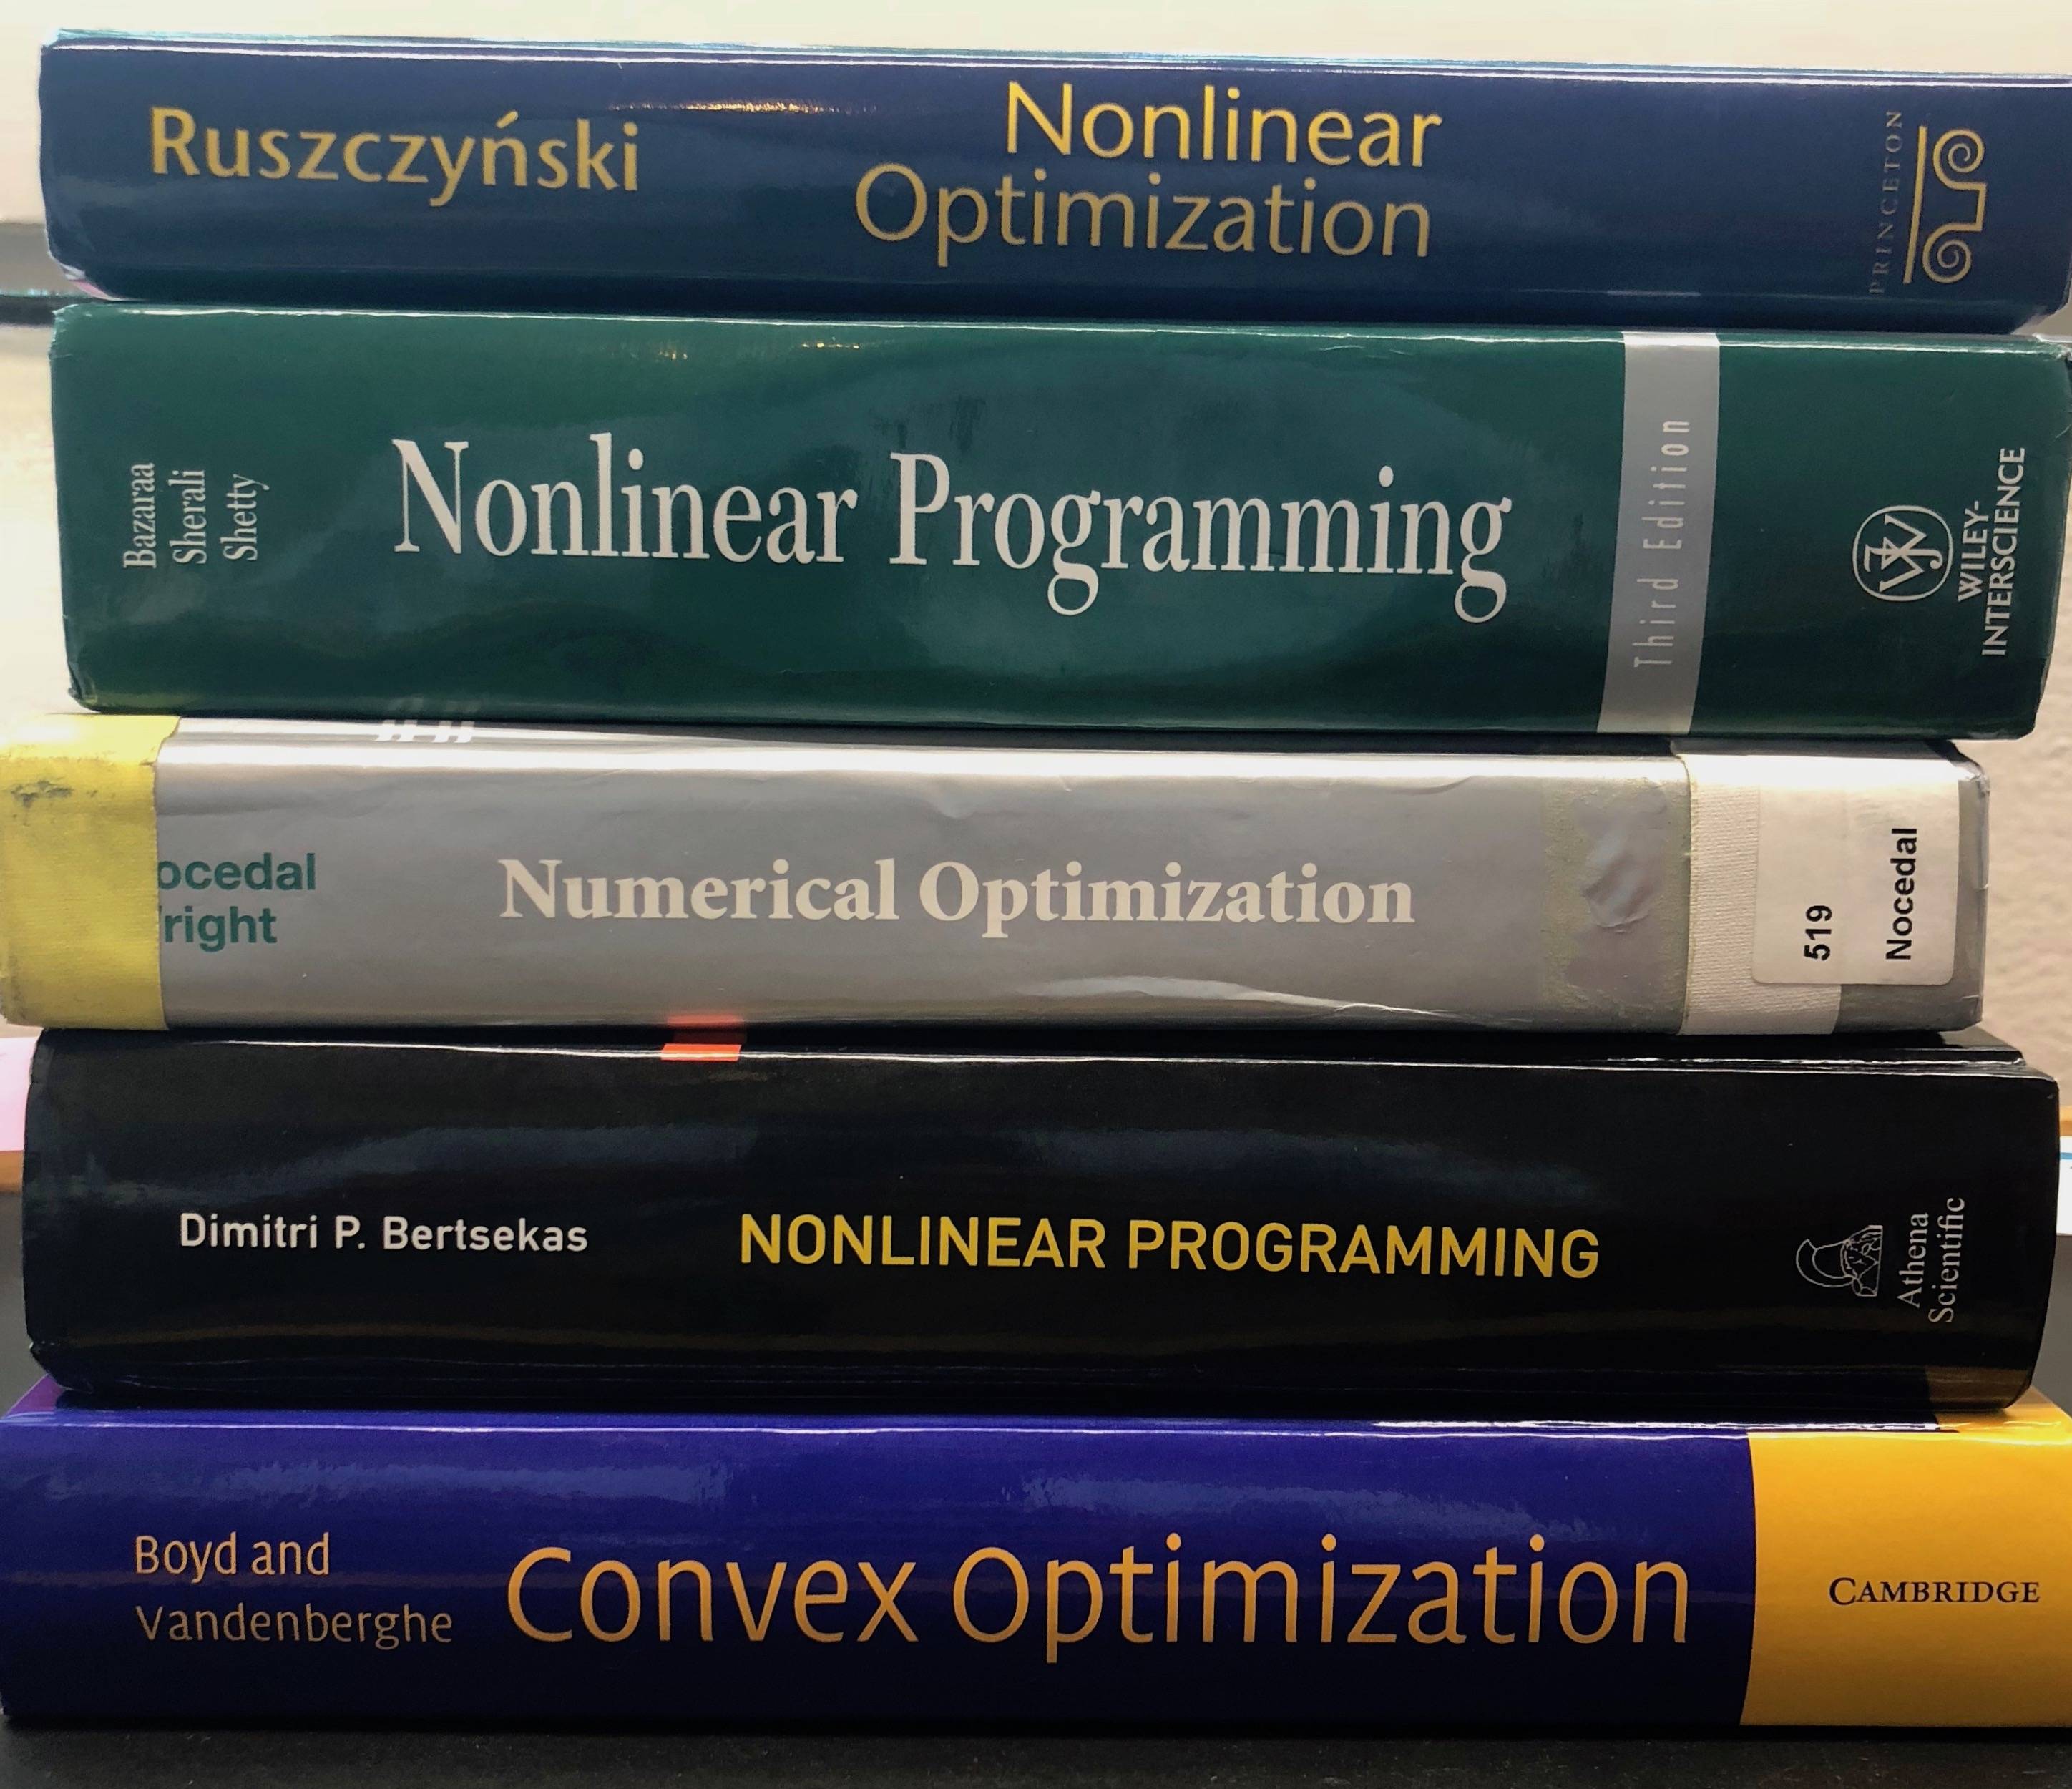
\includegraphics[scale=0.09]{Figures/Books.jpg}

\end{frame}


\subsection{Types of mathematical optimisation models}


	\begin{frame}{Types of programming}
	
	The \alert{simpler are the assumptions} which define a type of problems, the better are the \alert{methods to solve such problems}.
	
	\pause
	
	Some useful notation:
	
	\begin{itemize}[<+->]
		\item $x \in \reals^n$ - vector of (decision) variables $x_j$, $j = 1,\dots, n$;
		\item $f:\reals^n \rightarrow \reals \cup \braces{\pm \infty}$ - objective function;
		\item $X \subseteq \reals^n$ - ground set (physical constraints);
		\item $g_i, h_i : \reals^n \rightarrow \reals$ - constraint functions; 
		\item $g_i(x) \leq 0$ for $i = 1, \dots, m$ - inequality constraints;
		\item $h_i(x) = 0$ for $i = 1, \dots, l$ - equality constraints.
	\end{itemize}

\end{frame}


\begin{frame}{Types of programming}

	Our goal will be to solve variations of the general problem $P$:
	%
	\begin{align*}
		(P) :~ \mini \ & f(x) \\
		\st & g_i(x) \leq 0, i = 1, \dots, m\\
		& h_i(x) = 0, i = 1, \dots, l \\
		& x \in X.
	\end{align*}
	%
	\pause
	\vspace{-24pt}
	\begin{itemize}
	\item {\bf Linear programming (LP):} \alert{linear} $f(x) = c^\top x$ with $c \in \reals^n$; constraint functions $g_i(x)$ and $h_i(x)$ are \alert{affine} ($a_i^\top x - b_i$, with $a_i \in \reals^n$, $b \in \reals$); $X = \braces{ x \in \reals^n : x_j \geq 0, j =1,\dots,n}$.  
	\pause
	\item {\bf Nonlinear programming (NLP):} some (or all) of the functions $f, g_i$ or $h_i$ are \alert{nonlinear};
	\pause
	\item {\bf (Mixed-)integer programming ((M)IP):} LP where (some of the) variables are \alert{binary (or integer)}. $X \subseteq \reals^k \times \braces{0,1}^{n-k}$ 
	\pause 
	\item {\bf Mixed-integer\hspace{-1pt} nonlinear\hspace{-2pt} programming\hspace{-2pt} (MINLP):}\hspace{-1pt} {\small MIP\hspace{-3pt} +\hspace{-3pt} NLP.} 
	\end{itemize}

\end{frame}


\section{Applications}


\subsection{Resource allocation}


\begin{frame}{Resource allocation and portfolio optimisation}

	{\bf Problem statement.} Plan production that maximises return. Let
	\begin{columns}
		%% Juho
		\column{0.64\textwidth}
		\begin{itemize}
			\item {\small $I = \braces{1, \dots, i, \dots, M}$} resources; 
			\item {\small $J = \braces{1, \dots, j, \dots, N}$} products;
			\item $c_j$ - return per unit of product $j\in J$;
			\item $a_{ij}$ - resource $i\in I$ requirement for making product $j\in\hspace{-1pt} J$ ;
			\item $b_i$ - availability of resource $i\in I$; 
			\item $x_j$ - production of $j \in J$.
		\end{itemize}
		
		\column{0.4\textwidth}
		\pause
		\begin{align*}
			\maxi \ & \sum_{j \in J} c_jx_j \\
			\st & \sum_{j \in J}a_{ij}x_j \leq b_i, \forall i \in I\\
			& x_j \geq 0, \forall j \in J
		\end{align*} 
	\end{columns}
	\pause
	\vfill
	{\bf Remark:} 
	\vspace{-6pt}
	\begin{itemize}[<+->]
		\item notice that $\maxi f(x) = \mini - f(x)$;
		\item the base of \alert{most practical optimisation problems}; exploits mature LP technology.
	\end{itemize}

\end{frame}


\begin{frame}{Portfolio optimization}

	{\bf Problem statement.} Plan portfolio of assets to minimise exposition to risk. Let
	\begin{columns}
		\column{0.5\textwidth}
		\begin{itemize}
			\item {\small $J = \braces{1, \dots, j, \dots, N}$} assets;
			\item $\mu_j$ - expected relative return of asset $j \in J$;
			\item $\Sigma$ - covariance matrix;
			\item $\epsilon$ - minimum expected return;
			\item $x_j$ - position of asset $j \in J$
		\end{itemize}
	
		\column{0.4\textwidth}
		\pause
		\begin{align*}
			\mini \ &  x^\top\Sigma x  \\
			\st & \mu^\top x  \geq \epsilon\\
			& 0 \leq x_j \leq 1, \forall j \in J
		\end{align*} 
	\end{columns}
	\vfill
	\pause
	{\bf Remarks:} 
	\vspace{-6pt}
	\begin{itemize}
		\item The term $x^\top\Sigma x$ measures \alert{exposition to risk}. It is credited to Harry Markowitz (1952).
		\item Another important class: \alert{quadratic programming} (nonlinear).
	\end{itemize}

\end{frame}


\subsection{The pooling problem: refinery operations planning}


\begin{frame}{Refinery Operations Planning Problem}

	\begin{columns}
		\column{0.6\textwidth}
		{\bf Oil refinery operational planning}
		\begin{itemize}
			\item Goal is to maximize profit;
			\item Several possible configurations;
			\item \alert{Product property specifications} must be met;
		   \end{itemize}
		
		\column{0.4\textwidth}
		\begin{figure}
			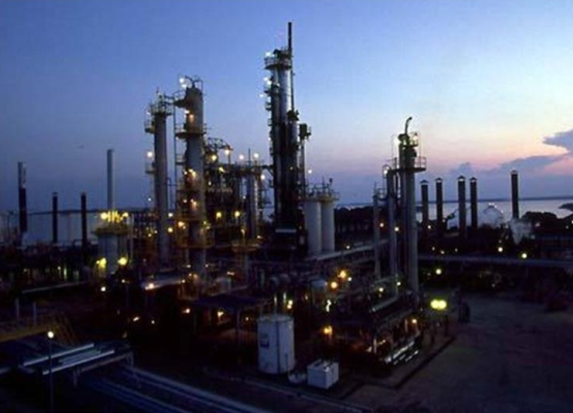
\includegraphics[width=\linewidth]{figures/Refinery.png}
		\end{figure}
	\end{columns}
	\pause
	\begin{columns}
		\column{0.6\textwidth}
		{\bf Model characteristics:}
			\begin{itemize}
				\item \alert{Bilinear (nonconvex) and mixed-integer};
				\item Large number of flows;
				\item Several nonlinear constraints.
		    \end{itemize}
		\column{0.4\textwidth}
		\begin{figure}
			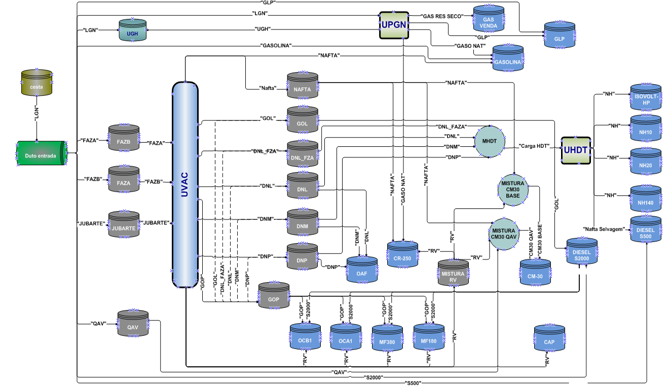
\includegraphics[width=\linewidth]{figures/RefinerySchema.png}
		\end{figure}
	\end{columns}

\end{frame}


\begin{frame}{Refinery Operations Planning Problem}

	\begin{columns}
		\column{0.65\textwidth}
		
		{\bf Objective:} maximize profit
		
		{\bf Variables:}
			\begin{itemize}
				\item Stream Flows {\footnotesize(crude, intermediate and final products)};
			    \item Storage;
			    \item Stream properties.
		    \end{itemize}
		\onslide<2->{
		
		{\bf Constraints}
			\begin{itemize}
				\item Mass balance;
			    \item Market features (supply and demand);
			    \item Unit capacities;
			    \item Stream property limits;
			    \item \alert{Calculation of mix properties (nonlinear)}.
		    \end{itemize}}
		\column{0.4\textwidth}
		% Second column
		\begin{figure}
			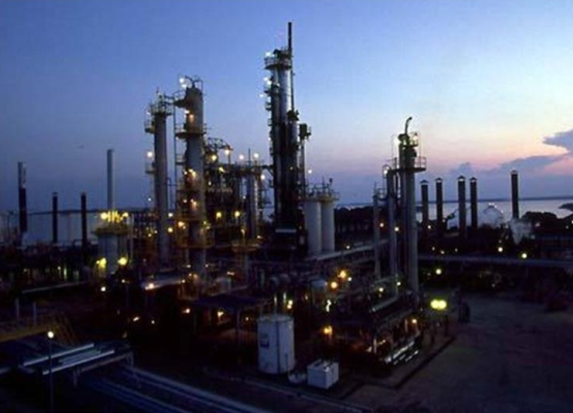
\includegraphics[width=\linewidth]{figures/Refinery.png}
		\end{figure}
		\begin{figure}
			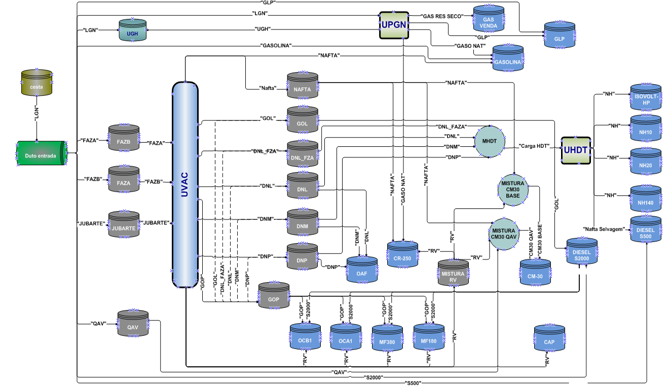
\includegraphics[width=\linewidth]{figures/RefinerySchema.png}
		\end{figure}
	\end{columns}
\end{frame}


\begin{frame}{Refinery Operations Planning Problem}

	The challenging aspect is how to model the calculation of product properties in a \alert{mix}. Let:
	
	\begin{itemize}
		\item $x_p$ be the volume of product $p \in P$ and
		\item $q_p$ the value of a given chemical property (sulphur content, octane content, viscosity...).
	\end{itemize}
	%
	In a given mix, mass and property balances are calculated as:
	
	\begin{columns}
		\column{0.5\textwidth}
		\centering
		\includegraphics[scale=0.6]{Figures/Mixer.pdf}
	%
		\column{0.5\textwidth}
		%
		\begin{align*}
		& x_A = x_B + x_C \\ 
		& q_A = \frac{q_Bx_B + q_Cx_C}{x_A}  
		\end{align*}
	%
	\end{columns}
	\pause
	{\bf Remarks:}
	\vspace{-6pt} 
	\begin{itemize}
		\item More complex mixes (such as nonlinear balances) might need to be considered.
		\item These are \alert{bilinear programming} problems (nonlinear).
	\end{itemize}
\end{frame}


\subsection{Robust optimisation}


\begin{frame}{Robust optimisation}
	
	Is a subarea of mathematical programming concerned with \alert{uncertainty in the input data}.
	
	It's a risk-averse perspective that seeks \alert{protection against variability}.
	
	\pause
	
	Consider the resource allocation problem under uncertainty:
	%
	\begin{align*}
		\maxi \ &  c^\top x \\
		\st & \tilde{a}_{i}^\top x \leq b_i, \forall i \in I\\
		& x_j \geq 0, \forall j \in J,
	\end{align*}
	
	where $\tilde{a}_{i}$ is a \alert{random variable}.

\end{frame}


\begin{frame}{Robust optimisation}

	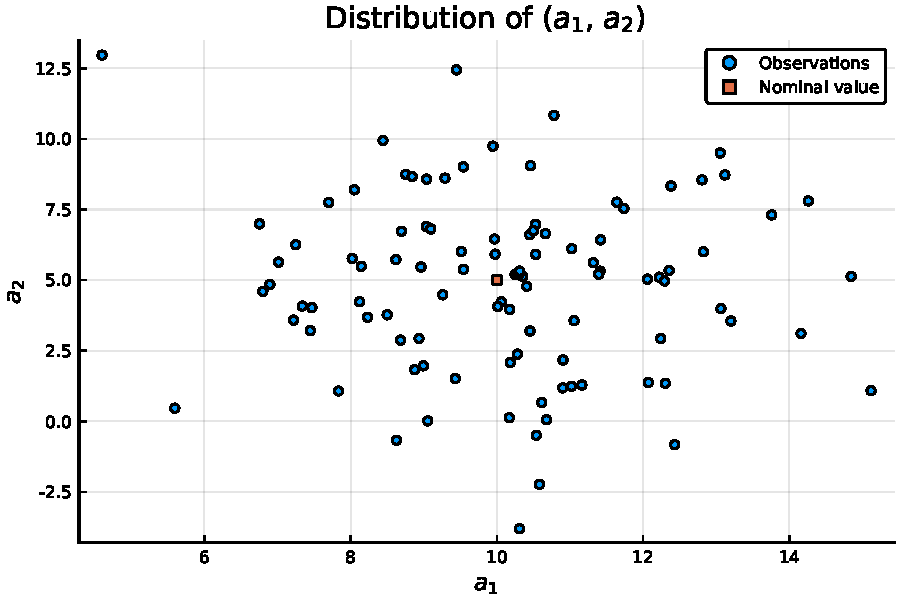
\includegraphics[width = 1\textwidth]{Figures/data_no_ellipsoid.pdf}

\end{frame}


\begin{frame}{Robust optimisation}

	Assume that,\hspace{-2pt} for\hspace{-2pt} any\hspace{-2pt} $i \in I$, $\tilde{a}_{i} \in \epsilon_i = \braces{\overline{a}_i + P_iu : ||u||_2 \leq \Gamma_i}$, where 
	\vspace{-6pt}
	
	\begin{itemize}
		\item $\overline{a}_{i}$ is the nominal (average) value; 
		%% Juho: I added the \epsilon here
		\item $P_i$ is the characteristic matrix of the ellipsoid $\epsilon$;
		\item $\Gamma_i$ is risk-aversion control parameter.
	\end{itemize}
	%
	\pause
	Then, the \alert{robust counterpart} can be stated as
	%
	\begin{align*}
		\maxi \ &  c^\top x \\
		\st & \maxi_{a_{i} \in \epsilon_i}\braces{a_i^\top x} \leq b_i, \forall i \in I\\
		& x_j \geq 0, \forall j \in J.
	\end{align*}
	\vspace{-6pt}
	%
	\pause
	Notice that 
	$$
	\maxi_{a_{i} \in \epsilon_i}\braces{a_i^\top x} = \overline{a}_i^\top x + \maxi_u\braces{u^\top P_i x : ||u||_2 \leq \Gamma_i} = \overline{a}_i^\top x + \Gamma_i||P_i x||_2 
	$$

\end{frame}


\begin{frame}{Robust optimisation}
	%
	The \alert{robust counterpart} can be equivalently stated as:
	\begin{align*}
		\maxi \ &  c^\top x \\
		\st & \overline{a}_i^\top x + \Gamma_i||P_i x||_2 \leq b_i, \forall i \in I\\
		& x_j \geq 0, \forall j \in J.
	\end{align*}
	%
	{\bf Remarks:}
	\begin{itemize}[<+->]
		\item In case data is available, $P_i$ can be obtained from the \alert{empirical covariance matrix};
		\item Values of $\Gamma_i$ can be drawn, for example, from a Chi-squared distribution. $\Gamma_i$ is sometimes called the \alert{budget of uncertainty}.
	\end{itemize}

\end{frame}


\begin{frame}{Robust optimisation}

	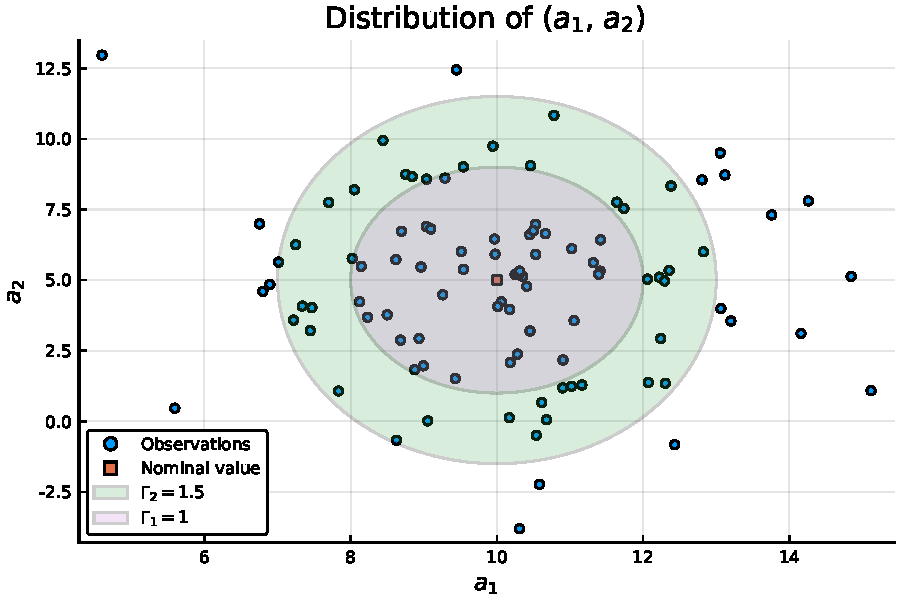
\includegraphics[width = 1\textwidth]{Figures/data_with_ellipsoid.pdf}

\end{frame}


\subsection{Classification: support vector machines}


\begin{frame}{Classification}

	Suppose we are given some data $D \subset \reals^n$ that can be \alert{separated} into two sets in $\reals^n$: $I^- = \braces{x_1,\dots, x_N}$ and $I^+ = \braces{x_1,\dots,x_M}$. 
	
	Each element in $D$ is an \alert{observation} of a given set of \alert{features}; belonging to either $I^-$ or $I^+$ defines a \alert{classification}.
	
	\pause
	Our task is to select a function $f:\reals^n \rightarrow \reals$ from a given family of functions such that
	$$
	f(x_i) < 0, \ \forall x_i \in I^- \text{ and } f(x_i) > 0, \ \forall x_i \in I^+.
	$$ 
	Typically, $f$ is selected as a \alert{linear classifier}, i.e., $f(x_i) = a^\top x_i - b$. 
	
	Of course, there is always the possibility of \alert{misclassification} and, therefore, we want to determine the \alert{best} possible classifier.

\end{frame}


\begin{frame}{Classification}

	\centering
	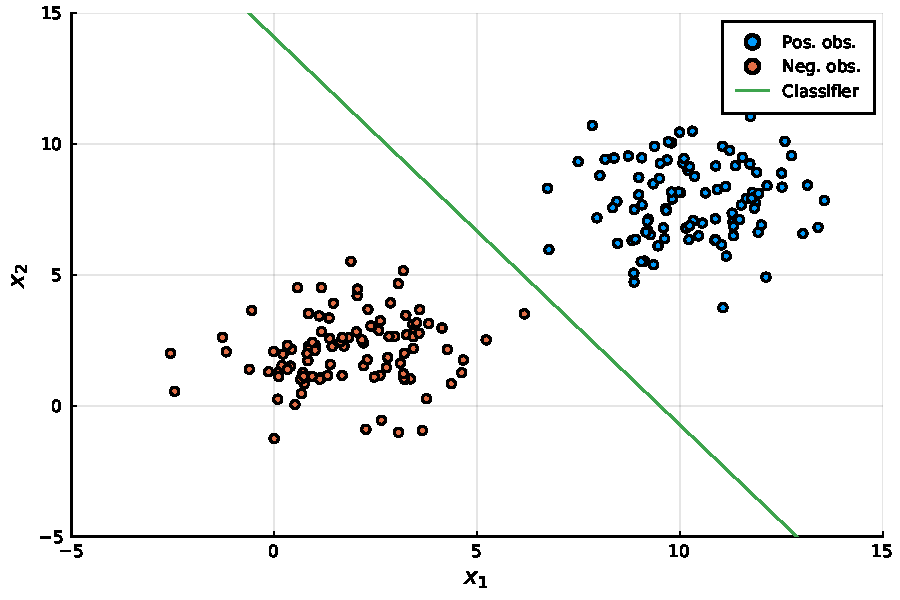
\includegraphics[width = \textwidth]{Figures/classes_with_classifier.pdf}

\end{frame}


\begin{frame}{Classification}

	Let us define the following \alert{error measures}:
	{\small
	\begin{align*}
		& e^-(x_i \in I^-; a, b) := \begin{cases} 0, \text{ if } a^\top x_i - b \leq 0, \\
	                                a^\top x_i - b, \text{ if } a^\top x_i - b > 0.
	                   \end{cases} \\
		& e^+(x_i \in I^+; a, b) := \begin{cases} 0, \text{ if } a^\top x_i - b \geq 0, \\
	                                b -  a^\top x_i, \text{ if } a^\top x_i - b < 0.
	                   \end{cases}                   
	\end{align*}}% 
	\pause
	Using \alert{slack variables} $u_i$, $i = 1,\dots,M$, and $v_i$, $i = 1,\dots,N$, to represent $e^-$ and $e^+$, the optimal classifier is obtained from:
	{\small
	\begin{align*}
		(LC) :~ \mini \ & \sum_{i=1}^M u_i + \sum_{i=1}^N v_i \\
		\st & a^\top x_i - b - u_i \leq 0, i = 1,\dots,M \\
		& a^\top x_i - b + v_i \geq 0, i = 1,\dots,N \\
		& ||a||_2 = 1\\
		&u_i \geq 0, i = 1,\dots,M; v_i \geq 0, i = 1,\dots,N; a \in \reals^n, b \in \reals.
	\end{align*}}
	%
%	{\bf Remark:} notice that $||a||_2 = 1$ avoids $(a,b) = (0,0)$. 
\end{frame}


\begin{frame}{Classification}

	In practice, we can enforce a \alert{slab} $S = \braces{-1 \leq a^\top x_i- b \leq 1}$ as a buffer to trade off the \alert{robustness} of the classifier to outliers. 
	
	Accordingly, we redefine our error measures as follows. 
	%
	\begin{align*}
	& e^-(x_i \in I^-; a, b) := 
	    \begin{cases} 0, \text{ if } a^\top x_i - b \leq -1, \\
	        a^\top x_i - b, \text{ if } a^\top x_i - b > -1.
	    \end{cases} \\
	& e^+(x_i \in I^+; a, b) := 
	    \begin{cases} 0, \text{ if } a^\top x_i - b \geq 1, \\
	        b -  a^\top x_i, \text{ if } a^\top x_i - b < 1.
	    \end{cases}                   
	\end{align*}
	%
	\pause
	$e^-$ and $e^+$ include \alert{misclassifications} and \alert{correct classifications that lie within $S$}. The latter are know as \alert{support vectors}.
	
	The \alert{width of $S$ is given by $2/||a||_2$}, which is the distance between the hyperplanes $a^\top x_i - b = -1$ and $a^\top x_i - b = 1$.
	
\end{frame}


\begin{frame}{Classification}

	The robust version of $LC$ incorporating this buffer becomes   
	%
	\begin{align*}
		\mini \ & \sum_{i=1}^M u_i + \sum_{i=1}^N v_i + \gamma||a||_2^2\\
		\st & a^\top x_i - b - u_i \leq -1, \ i = 1,\dots,M \\
		& a^\top x_i - b + v_i \geq -1, \ i = 1,\dots,N \\
		& u_i \geq 0, i = 1,\dots,M; v_i \geq 0, i = 1,\dots, N; \\
		& a \in \reals^n, b \in \reals.
	\end{align*} 
	\pause
	{\bf Remarks:}
	\vspace{-6pt}
	\begin{itemize}[<+->]
		\item The parameter $\gamma$ controls the \alert{trade-off} between the width of the slab $S$ and the number of observations within the slab.
		\item This quadratic programming problem is known in the machine learning literature as \alert{support vector machine} (SVM).
	\end{itemize}

\end{frame}


\begin{frame}{Classification}

	\centering
	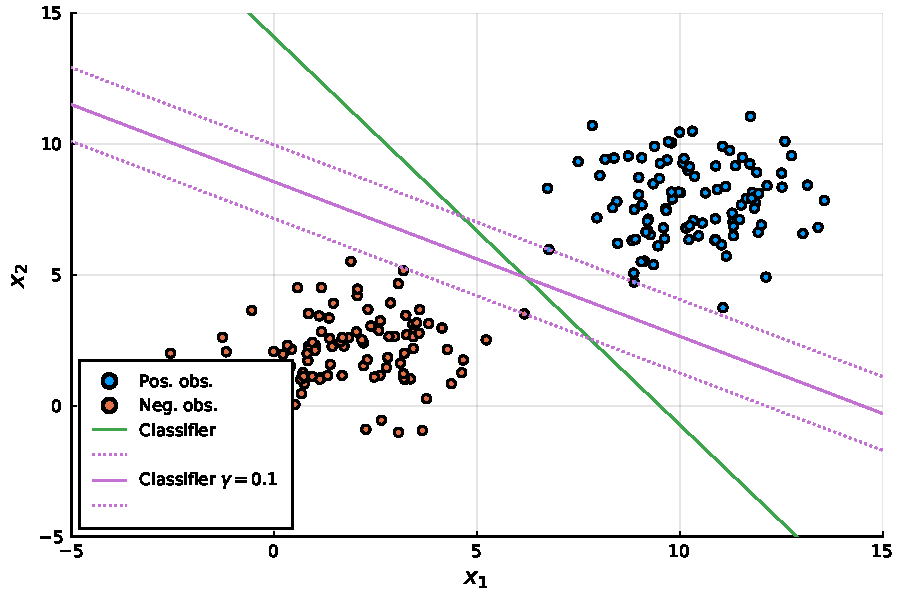
\includegraphics[width = \textwidth]{Figures/classes_with_robust_classifier.pdf}

\end{frame}


\end{document}